\newpage
\chapter{Инсталация и стартиране}
\label{chapter01}

Тъй като програмният продукт R се разработва под формата на софтуер с отворен код, то употребата му с не търговска цел не изисква заплащане. За работа с R е достатъчно да се инсталира основния пакет, въпреки това съществува и интегрирана среда за разработка наречена R Studio. За нуждите на учебното помагало ще бъде използван само основният пакет. Всеки желаещ да разшири уменията си с използването на интегрираната среда за разработка, би могъл самостоятелно да разучи възможностите й.

\section{Изтегляне на инсталационните файлове}

\begin{figure}[h!]
  \centering
  
\includegraphics[width=1.0\linewidth]{pic0001}
  \caption{Начална уеб страница на продукта}
\label{fig:pic0001}
\end{figure}
\FloatBarrier

Както множество софтуерно продукти и R е достъпен за изтегляне от уеб страницата на продукта в Интернет (Фиг. \ref{fig:pic0001}) с адрес: http://www.r-project.org/ 

\begin{figure}[h]
  \centering
  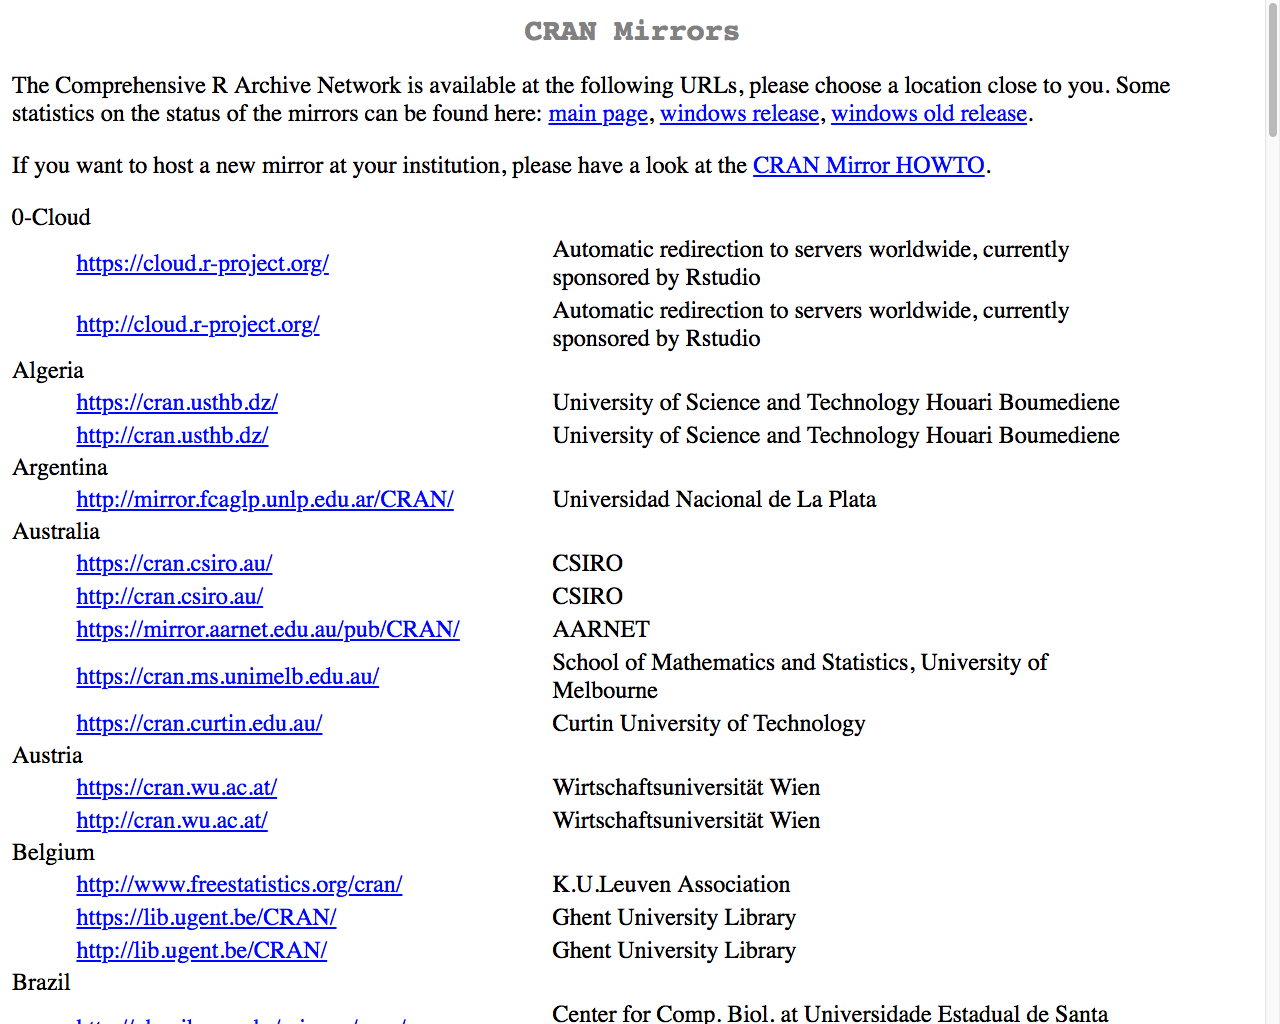
\includegraphics[width=1.0\linewidth]{pic0002}
  \caption{Списък със сървъри за изтегляне}
\label{fig:pic0002}
\end{figure}
\FloatBarrier
В раздела за изтегляне са посочени множество активни връзки към различни географски локации (Фиг. \ref{fig:pic0002}).

\begin{figure}[h]
  \centering
  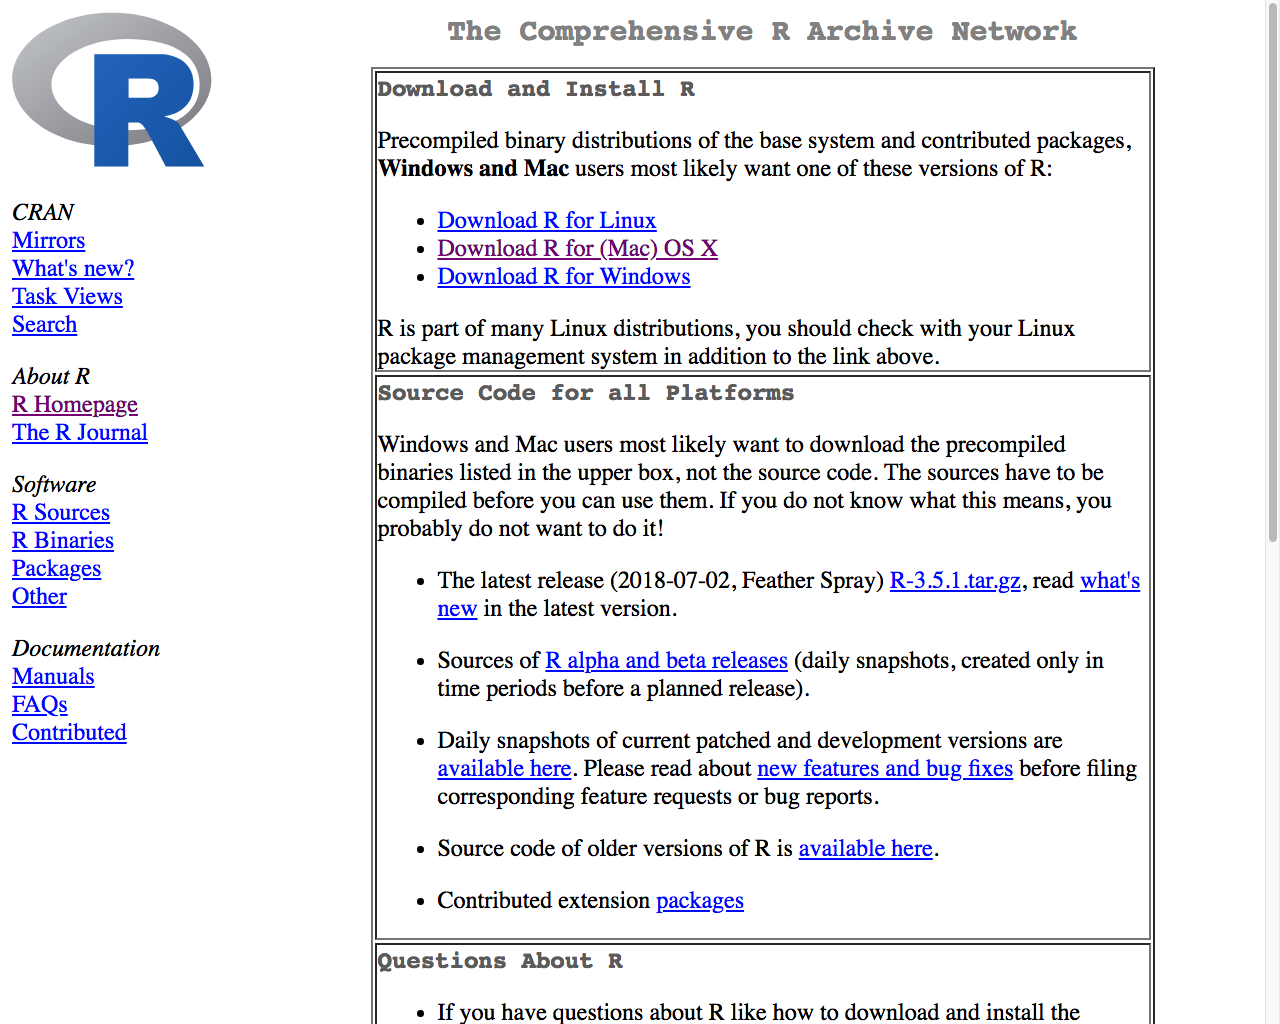
\includegraphics[width=1.0\linewidth]{pic0003}
  \caption{Избор на подходящата за операционната система инсталация}
\label{fig:pic0003}
\end{figure}
\FloatBarrier

Както множество софтуерни продукти с отворен код, така и R се разпространява за трите най-популярни операционни системи (Фиг. \ref{fig:pic0003}).

\begin{figure}[h]
  \centering
  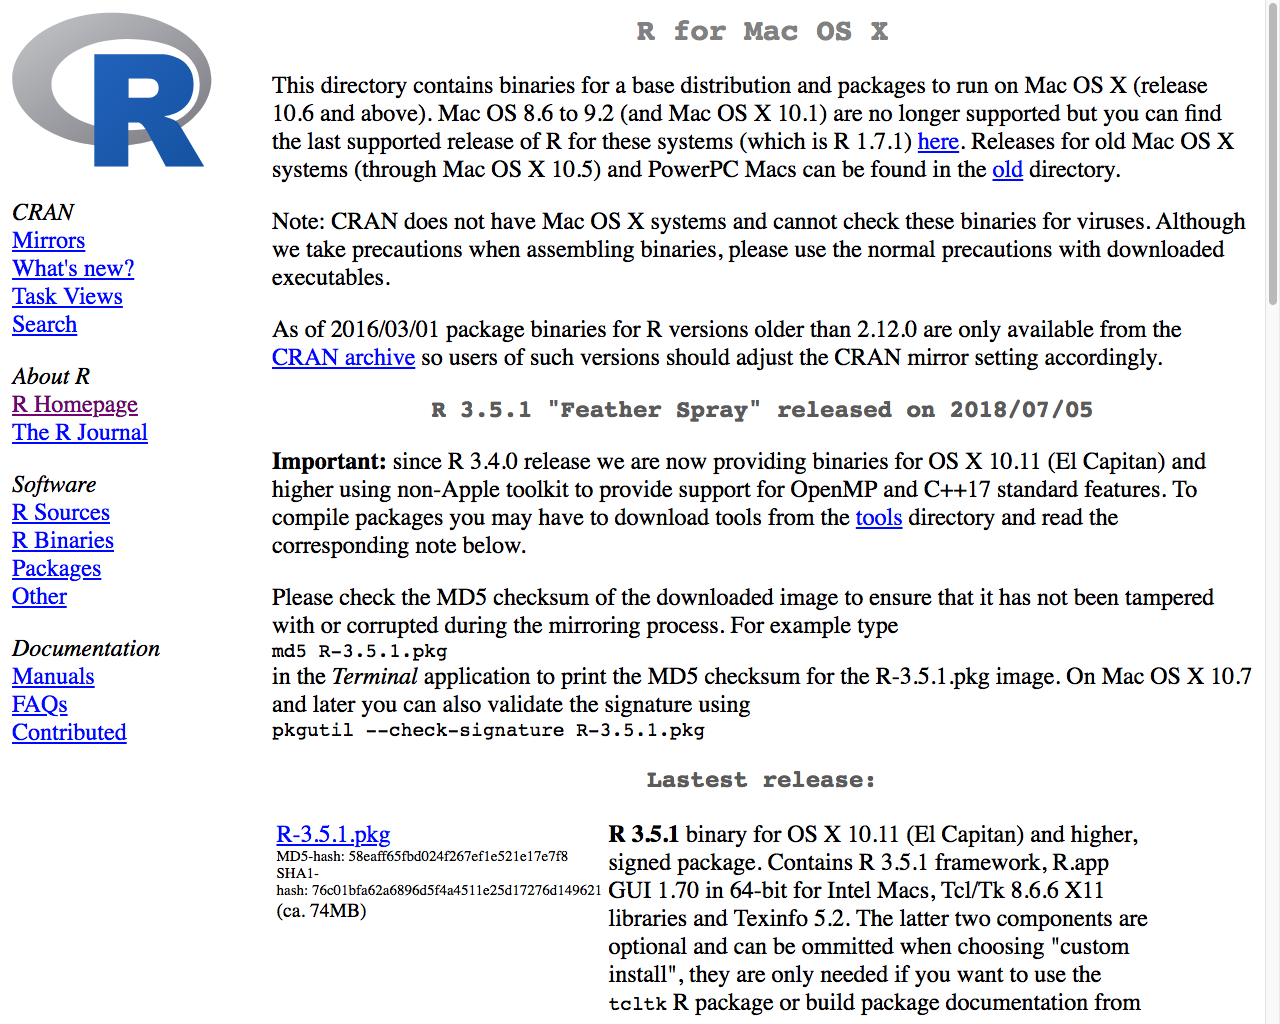
\includegraphics[width=1.0\linewidth]{pic0004}
  \caption{Избор на версия за изтегляне}
\label{fig:pic0004}
\end{figure}
\FloatBarrier

Добра практика е при работата със софтуерни продукти, които се разпространяват като отворен код, винаги да се използва най-новата стабилна версия. В случая, за операционната система Mac OS X (Фиг. \ref{fig:pic0004}), това е версията 3.5.1, която е налична под формата на инсталационне файл R-3.5.1.pkg (Фиг. \ref{fig:pic0003}).

\begin{figure}[h]
  \centering
  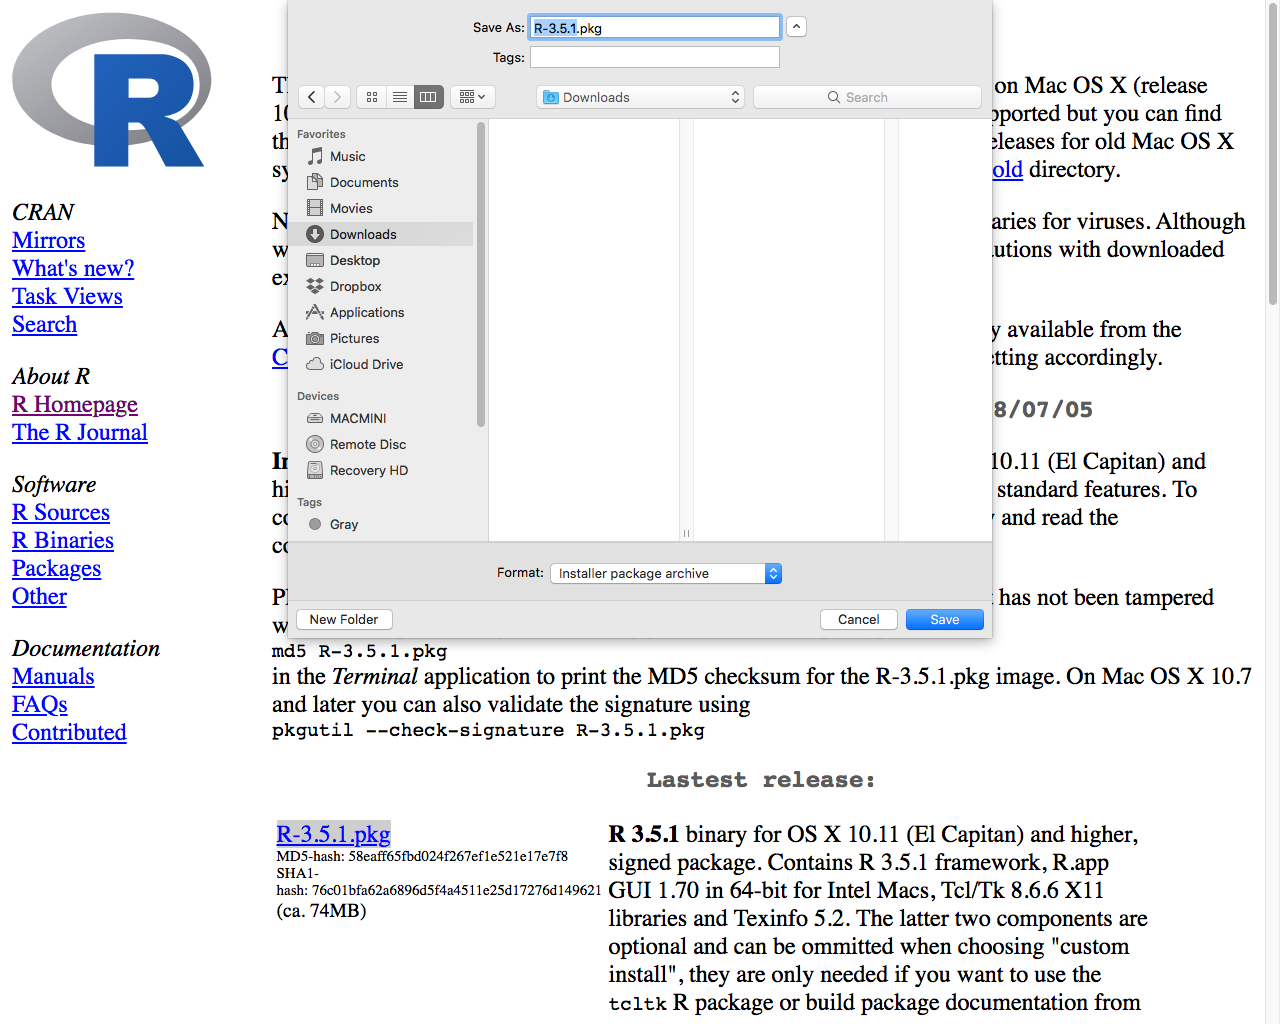
\includegraphics[width=1.0\linewidth]{pic0005}
  \caption{Запазване на инсталационния файл}
\label{fig:pic0005}
\end{figure}
\FloatBarrier

\section{Инсталация}

За всяка от операционните системи е достатъчно потребителят да следва инструкциите и инсталацията протича безпроблемно по указаните стъпки. 

\begin{figure}[h]
  \centering
  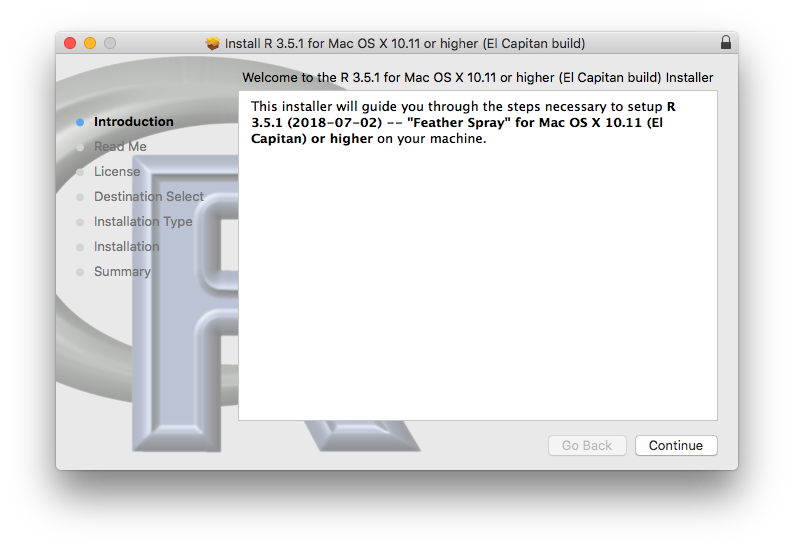
\includegraphics[width=1.0\linewidth]{pic0006}
  \caption{Активиране на инсталатора}
\label{fig:pic0006}
\end{figure}
\FloatBarrier

С двойно щракване на мишката се активира инсталатора (Фиг. \ref{fig:pic0006}). След което следва екран с подробности за самата инсталация (Фиг. \ref{fig:pic0007}).

\begin{figure}[h]
  \centering
  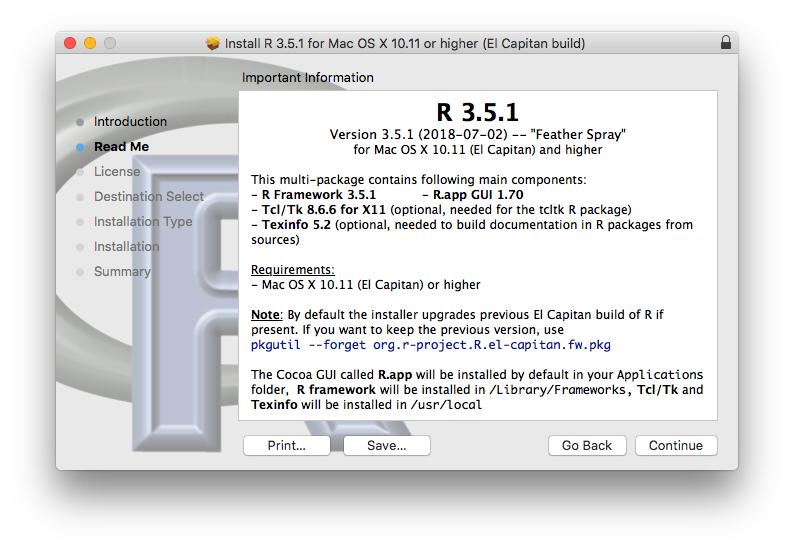
\includegraphics[width=1.0\linewidth]{pic0007}
  \caption{Подробности за инсталацията}
\label{fig:pic0007}
\end{figure}
\FloatBarrier

От съществено значение е потребителите на продукти с отворен код да са добре запознати с условията при които те получават продуктите, особено когато е без заплащане. Поради тази причина, потребителят трябва изрично да се съгласи с условията на лиценза под който се разпространява продуктът R (Фиг. \ref{fig:pic0008,fig:pic0009}).

\begin{figure}[h]
  \centering
  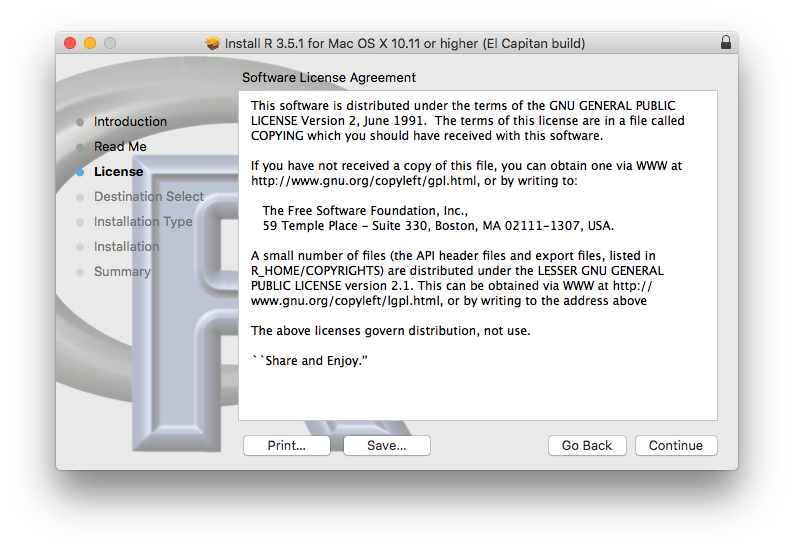
\includegraphics[width=1.0\linewidth]{pic0008}
  \caption{Лицензно споразумение за ползване}
\label{fig:pic0008}
\end{figure}
\FloatBarrier

\begin{figure}[h]
  \centering
  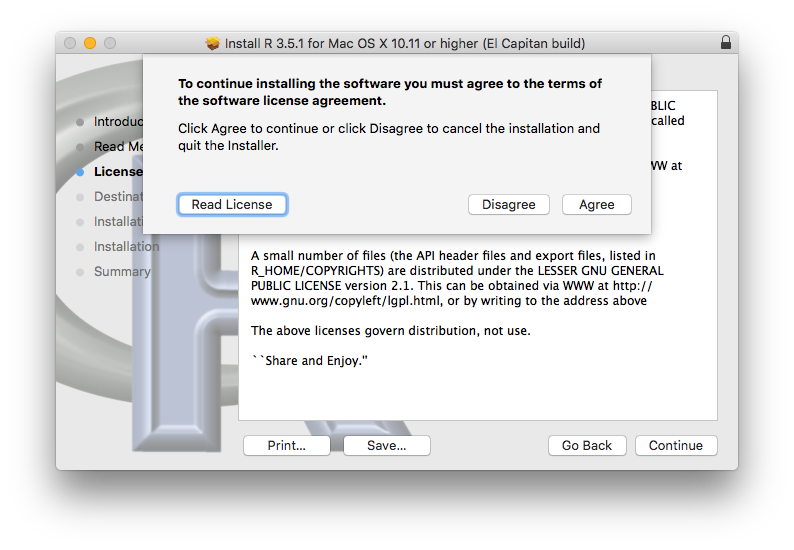
\includegraphics[width=1.0\linewidth]{pic0009}
  \caption{Изрично съгласие}
\label{fig:pic0009}
\end{figure}
\FloatBarrier

\begin{figure}[h]
  \centering
  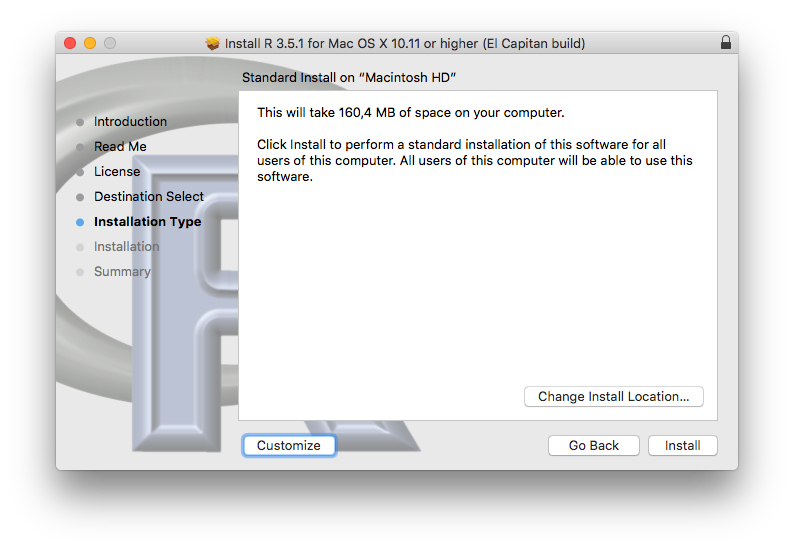
\includegraphics[width=1.0\linewidth]{pic0010}
  \caption{Информация за директорията и използваното дисково пространство}
\label{fig:pic0010}
\end{figure}
\FloatBarrier

При желание е възможно да бъде подменена инсталационната директория (Фиг. \ref{fig:pic0010}).

\begin{figure}[h]
  \centering
  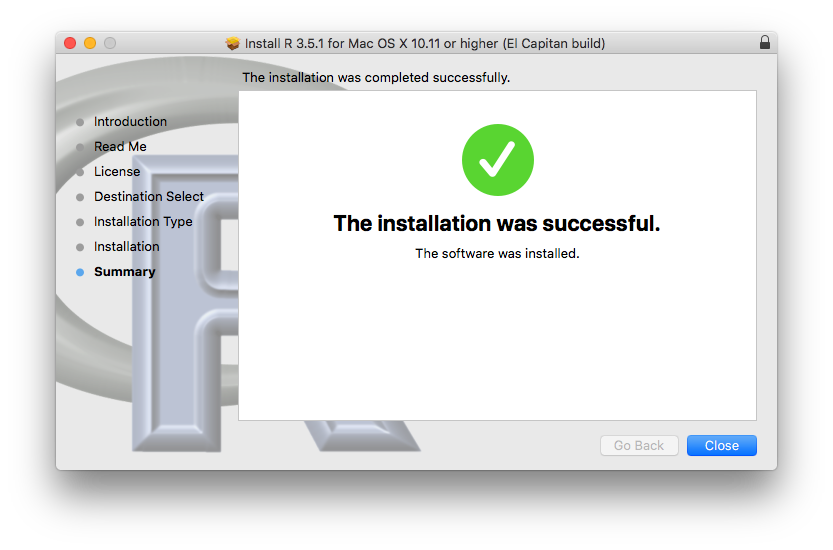
\includegraphics[width=1.0\linewidth]{pic0011}
  \caption{Успешно приключване на инсталацията}
\label{fig:pic0011}
\end{figure}
\FloatBarrier

Инсталацията приключва със съобщение за успешно изпълнение (Фиг. \ref{fig:pic0011}).

\section{Работа в режим на команди}

Инсталаторът създава икона за стартиране на R командния интерпретатор.

\begin{figure}[h]
  \centering
  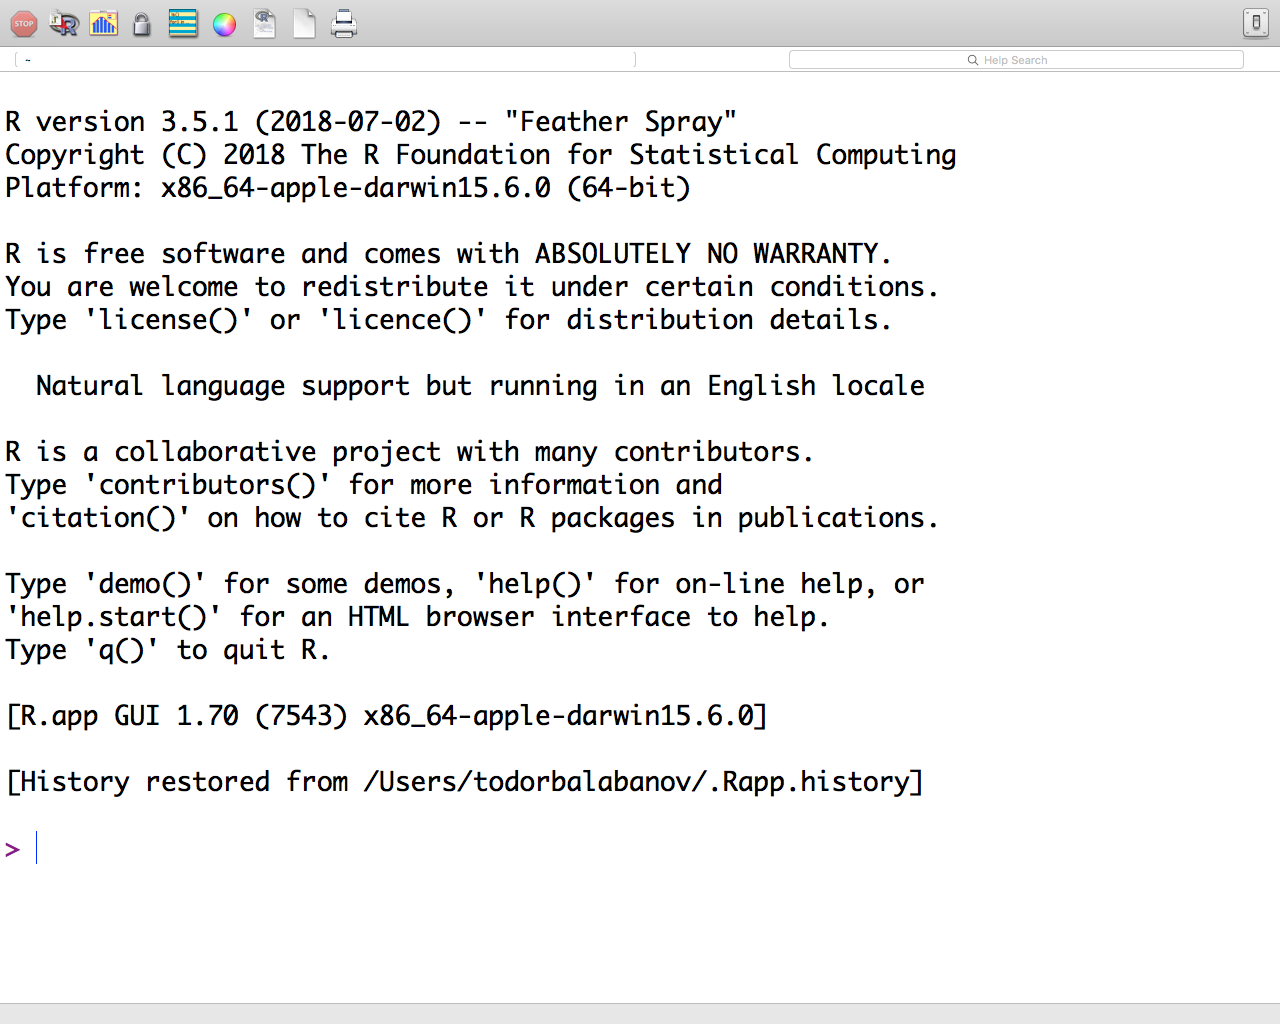
\includegraphics[width=1.0\linewidth]{pic0012}
  \caption{Основен прозорец на продукта}
\label{fig:pic0012}
\end{figure}
\FloatBarrier

При успешна инсталация и стартиране, потребителят получава достъп до прозорец служещ като команден интерпретатор (Фиг. \ref{fig:pic0012}).

\begin{figure}[h]
  \centering
  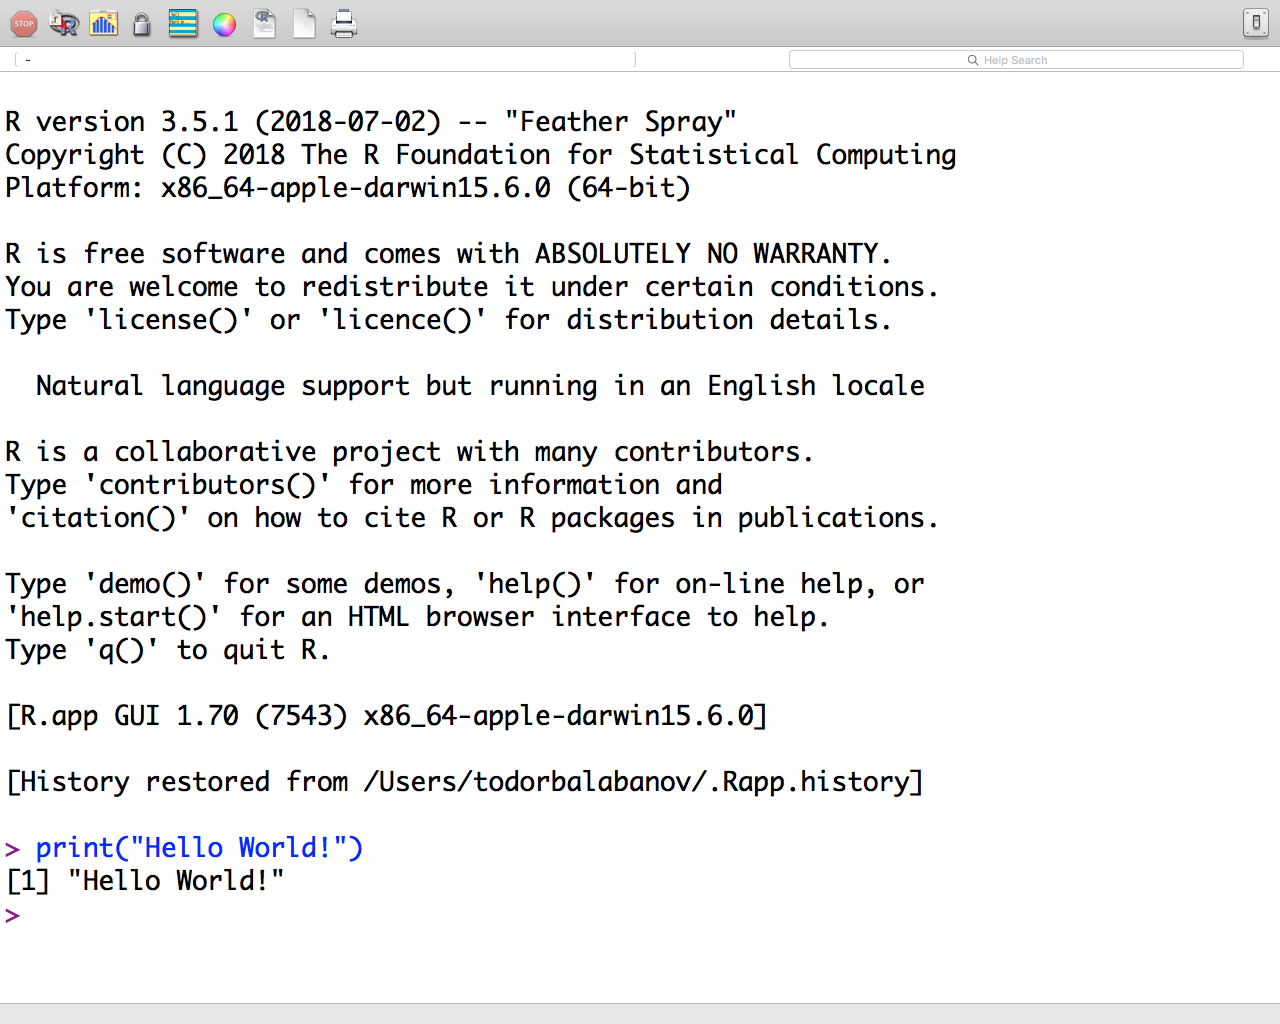
\includegraphics[width=1.0\linewidth]{pic0013}
  \caption{Изпълнение на команда за печат}
\label{fig:pic0013}
\end{figure}
\FloatBarrier

При правилно работеща инсталация изписването на командата за печат би дала резултата показан на Фиг. \ref{fig:pic0013}.